\documentclass{article}

\usepackage{fullpage}
\usepackage{amssymb}
\usepackage{graphicx}
\usepackage{psfrag}
\usepackage{algorithm}
\usepackage{algorithmic}
\usepackage{tikz}
\usetikzlibrary{intersections}

\newtheorem{lemm}{Lemma}
\newtheorem{defi}{Definition}
\newenvironment{proof}{\noindent{Proof:}}{}

\newcommand{\intersection}[2]{\langle #1, #2\rangle}

\newcommand{\creategrid}[2]{%
  \draw[step=1] (0,0) grid (#1,#2);%
%
  \foreach \x in {1,...,#1}%
    \draw (\x - 0.5, -0.5) node {\x};%
%
  \foreach \y in {1,...,#2}%
    \draw (-0.5, \y - 0.5) node {\y};%
}%
\newcommand{\drawobstacle}[2]{%
\draw[fill=black] (#1,#2) rectangle +(-1,-1);
}%


\begin{document}

\title{An Optimal Any-Angle Pathfinding Algorithm}
\maketitle

\section{Introduction}
\section{Introduction}
Any-angle pathfinding is a navigation problem which appears in robotics
and computer video games. It involves finding a shortest path between an 
arbitrary pair of points on a two-dimensional grid map but asks that 
movement along the path is not artificially constrained to the points of 
the grid.  Within the game development community a simple and popular 
solution exists known as \emph{string pulling}~\cite{pinter01,botea04}.
The idea is to compute a grid-optimal path in the first
instance and smooth the result as part of a post-processing step that improves
both its length and aesthetic appeal. String pulling has two disadvantages: 
(i) it requires more computation than just finding a path (ii)
it only yields approximately shortest paths.

A number of algorithms improve on string-pulling by integrating post-processing
into node-expansion during search. Field D*~\cite{ferguson05} uses linear 
interpolation to smooth paths one grid cell at a time. 
Theta*~\cite{nash07} 
%and its variants %\cite{%nash09, nash10,munoz12}
introduces a shortcut each time a successful line-of-sight check
is made from the parent of the current node to any of its successors.
Meanwhile, Block A*~\cite{yap11} employs during search a pre-computed database
of optimal Euclidean distances between pairs of points in a localised area.
Each of these approaches improves on string pulling in terms of solution 
quality and, in many cases, running time. Unfortunately none are optimal.
Accelerated A*~\cite{sislak09b} is an any-angle algorithm that is conjectured 
to be optimal but for which no strong theoretical argument is made. Similar to Theta*, 
it differs primarily in that line-of-sight checks are performed from a set
of expanded nodes rather than a single ancestor. The size of the set is only
loosely bounded and, for challenging problems, can include a large proportion
of nodes on the Closed List.

%
% Its main disadvantage is that,
%for challenging problems, it can perform line-of-sight checks against a large 
%proportion of nodes on the Closed List.
%
%Theta*~\cite{nash07} and its variant~\cite{%nash09,
%nash10} improve things 
%by integrating post-processing into node expansion during search. Their 
%idea involves updating a node's parent label following a successful line-of-sight
%check to a previously expanded ancestor node.
%Another approach, Block A*~\cite{yap11}, avoids line-of-sight checks entirely 
%by precomputing a database of exact costs between pairs of points in a localised area.
%Both Theta* and Block A* improve on the running time and 
%solution quality of string pulling but neither guarantees optimality.
%Despite this, a number of exact solutions for the problem do exist.
%\\
%In computational geometry a problem similar to any-angle pathfinding exists 
%which has been very well studied: finding Euclidean shortest paths among 
%polygonal obstacles in the plane.
Tangent Graphs~\cite{liu92} and Visibility Graphs~\cite{lozanoperez79} are 
optimal techniques that can solve a generalised form of the any-angle pathfinding 
problem. Their primary disadvantage is that each such graph requires quadratic 
space in the worst case and must be computed offline.
Other exact approaches are based on the 
Continuous Dijkstra~\cite{mitchell87} paradigm.
The most efficient of these algorithms~\cite{hershberger99} pre-computes a 
planar subdivision of the map that can be used to extract a path in just
logarithmic time. Unfortunately the precomputation assumes the starting location
does not change.

In this work we introduce a new approach to any-angle pathfinding 
which addresses many of the shortcomings associated with existing research.
Our method, Anya, bears some similarity with Continuous Dijkstra: 
instead of searching over the individual nodes of the grid we 
search over contiguous sets of states that form intervals.
Each interval has a representative point used to derive an $f$-value
and each is projected from one row of the grid onto another until the 
goal is reached.
%instead of searching over individual states from the grid we consider
%contiguous sets of states together as an interval. From each interval we select a 
%representative point that is used to derive an $f$-value for the set.
%Intervals are associated with corner points and projected from one 
%row of the grid onto another until the goal is reached.
Anya does not rely on any precomputation, does not introduce any
memory overheads (beyond what is required by e.g. A*) and always finds 
an optimal any-angle path.
%compares favourably with existing research: (i)
%it always finds an optimal any-angle path (ii) 
%it does not rely on any precomputation (iii) 
%it does not introduce any memory overheads 
%beyond those required by a pathfinding algorithm such as A*.

%http://www.valvesoftware.com/publications/2009/ai_systems_of_l4d_mike_booth.pdf
%http://digestingduck.blogspot.com.au/2010/03/simple-stupid-funnel-algorithm.html


\section{Problem Definitions}
A \emph{grid} is a matrix 
of \emph{traversable} and \emph{non-traversable} \emph{tiles}.  
Formally, a grid $G$ is a $W \times H$ vector of boolean, 
where $G[x,y] = \top$ if the tile $[x,y]$ is traversable 
and $\bot$ if it is not.  
An intersection $(x,y)$ ($x \in \{0,\dots,W\}$ and $y \in \{0,\dots,H\}$) 
is the point that is common to the tiles 
$[x-1,y-1]$, $[x,y-1]$, $[x,y]$, and $[x-1,y]$, 
where the tiles outside the grid are assumed non traversable.  

A \emph{corner} is an intersection 
such that only one of its four squares is non-traversable.  
Intersection $i'$ is \emph{visible} from intersection $i$ 
iff the segment $(i,i')$ crosses only traversable tiles 
or borders non-traversable tiles and traversable tiles.  
Without loss of generality, 
we assume that if the segment $(i,i')$ crosses a corner 
(besides $i$ and $i'$), 
then intersection $i'$ is not visible from intersection $i$.  

An \emph{any-angle path} $\pi$ is a sequence $p_1,\dots,p_k$ 
of points that are visible from each other.  
The \emph{length} of path $\pi$ 
is the cumulative distance of every pair of points in the path, 
i.e., $d(p_1,p_2) + d(p_2,p_3) + \dots + d(p_{k-1},p_k)$, 
where $d((x,y),(x',y')) = \sqrt{(x-x')^2 + (y-y')^2}$ 
is the (uniform) Euclidian distance between the two points.  

A \emph{turning point} in path $\pi$ 
is defined as i) either a corner 
%or ii) the first or last point of the path 
or ii) a point $p_l$ of the path 
such that the segments $(p_{l-1},p_l)$ and $(p_l,p_{l+1})$ form an angle.  
It is easy to see that for any path $\pi$ 
that includes a non-turning point $p$ 
(besides the first and last points), 
the sequence of points $\pi \setminus p$ 
(i.e., where point $p$ has been removed from $\pi$) 
is also a path of same length as $\pi$.  
Therefore, we will only consider paths 
that are exclusively composed of turning point.  

\begin{lemm}
  Given two points $p$ and $p'$, 
  any turning point in the optimal any-angle path between $p$ and $p'$ 
  is a corner.  
\end{lemm}

\begin{proof}
{
  Assume an optimal any-angle path $\pi = (p_1,\dots,p_k)$ 
  that includes a turning point $p_l$ ($l \not\in \{0,k\}$) 
  which is not a corner.  
  We will prove that $\pi$ is suboptimal 
  which, by contradiction, will prove the lemma.  
  
  If $p_{l+1}$ is visible from $p_{l-1}$, 
  then  $\pi \setminus p_l$ is a path 
  which is strictly shorter than $\pi$.  
  Hence $\pi$ is suboptimal.  

  If $p_{l+1}$ is not visible from $p_{l-1}$, 
  then let $p'_l$ be a point from the segment $(p_l,p_{l+1})$ 
  that i) is visible from $p_{l-1}$ 
  and ii) is different from $p_l$.  
  Because $p_l$ is not a corner, 
  then such a $p'_l$ exists.  
  The subpath $(p_{l-1},p_l,p'_l,p_{l+1})$ 
  is as long as $(p_{l-1},p_l,p_{l+1})$ 
  since $p'_l$ lies between $p_l$ and $p_{l+1}$.  
  The triangle inequality, however, 
  tells us that $(p_{l-1},p'_l,p_{l+1})$ is shorter than the subpath, 
  which proves that $\pi$ is suboptimal.

  This is illustrated on Figrure~\ref{fig::corner}  
  where the point $p'_l$ is chosen 
  as close as possible from the corner $c$.  
}

\begin{figure}[ht]
  \begin{center}
    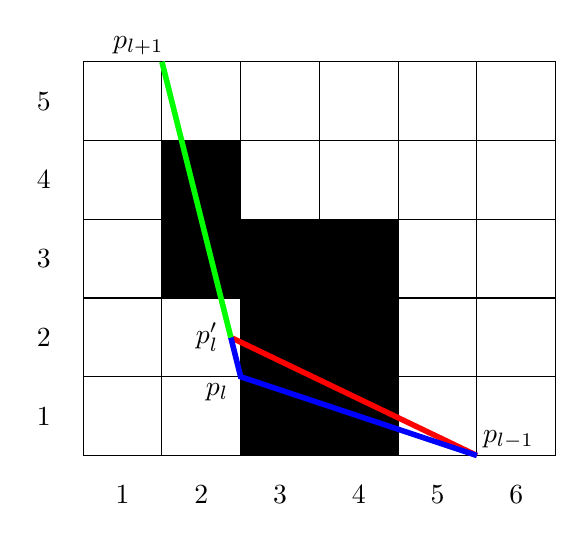
\begin{tikzpicture}

\creategrid{6}{5}

%\drawobstacle{2}{5}
\drawobstacle{2}{4}
\drawobstacle{2}{3}
\drawobstacle{3}{3}
\drawobstacle{3}{2}
\drawobstacle{3}{1}
\drawobstacle{4}{3}
\drawobstacle{4}{2}
\drawobstacle{4}{1}

\coordinate (plm1)   at (5,0);
\coordinate (pl)     at (2,1);
\coordinate (plp1)   at (1,5);
\coordinate (redpathdirection) at (0,2.4); % Actually, further away
\coordinate (actualcorner) at (3,1); 
\path[name path=uppath] (pl) -- (plp1);
\path[name path=shortcut] (plm1) -- (redpathdirection);
\draw[name intersections={of=uppath and shortcut, by=plp'}];

\draw[red, line width=2pt]   (plm1) -- (plp');
\draw[blue, line width=2pt]  (plm1) -- (pl) -- (plp');
\draw[green, line width=2pt] (plp1) -- (plp');

\draw (plm1) +(0.4,0.2) node {$p_{l-1}$};
\draw (pl) +(-0.3,-0.2)   node {$p_{l}$};
\draw (plp1) +(-0.3,0.2) node {$p_{l+1}$};
\draw (plp') +(-0.3,0) node {$p'_l$};
%\draw (actualcorner) +(-0.3,0.3) node {$c$};

\end{tikzpicture}

  \end{center}
  \caption{Illustration that making the path turn 
  outside a corner is suboptimal: 
  the blue and green path is longer than the red and green path.}
  \label{fig::corner}
\end{figure}

\end{proof}

Note that a similar observation has been made for geodesic paths \cite{mitchell87}.  

% EOF


\section{Principle}
\section{Principle Of Anya}
Consider the any-angle instance depicted in Figure~\ref{fig::ex1}. 
The start point is $n_1 = (2, 0)$ and the target
point is $n_2 = (3, 4)$.  The best online algorithm for solving such
problems, to date, is Theta*~\cite{nash07}; a method which computes
an any-angle path by only considering the set of discrete points from 
the grid. 
Each time such a point is reached Theta* ``pulls the string''.  
Thus when node $n_2$ is generated its $g$-value is not
the length of the grid-constrained path from $n_1$ to $n_2$
but rather the length of the direct path $\langle n_1, n_2 \rangle$.

%\begin{figure}[tb]
% \begin{minipage}[b]{\0.45\linewidth}
%  \begin{center}
%    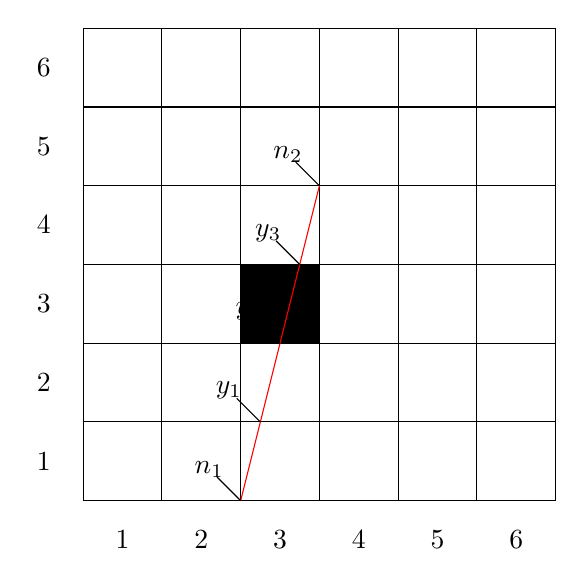
\begin{tikzpicture}

\creategrid{6}{6}

\drawobstacle{3}{3}

\coordinate (n1) at (2,0);
\coordinate (n2) at (3,4);

\path[name path=direct] (n1) -- (n2);
\path[name path=row 1] (0,1) -- (6,1);
\path[name path=row 2] (0,2) -- (6,2);
\path[name path=row 3] (0,3) -- (6,3);
\draw[name intersections={of=direct and row 1,by=y1}];
\draw[name intersections={of=direct and row 2,by=y2}];
\draw[name intersections={of=direct and row 3,by=y3}];

\draw[red] (n1) -- (n2);

\draw (n1) ++(-0.4,0.4) node {$n_1$} + (0.1,-0.1) -- (n1);
\draw (n2) ++(-0.4,0.4) node {$n_2$} + (0.1,-0.1) -- (n2);
\draw (y1) ++(-0.4,0.4) node {$y_1$} + (0.1,-0.1) -- (y1);
\draw (y2) ++(-0.4,0.4) node {$y_2$} + (0.1,-0.1) -- (y2);
\draw (y3) ++(-0.4,0.4) node {$y_3$} + (0.1,-0.1) -- (y3);

\end{tikzpicture}

%  \end{center}
%  \caption{Example of an any-angle path}
%  \label{fig::ex1}
%  \end{minipage}
%\end{figure}

The problem with this approach is that the solution-cost estimate
(or $f$-value), from a parent node to each of its successors, may 
not be monotonically increasing.  The monotone condition is
necessary to guarantee that an optimal solution, if one exists, is always found.
For instance: Theta* can generate $n_2$ from the intermediate point $p = (3,3)$.
When $p$ is expanded we have $f(p) = d(n_1, p) + h(p, n_2) = 4.16$. 
To satisfy the monotone condition we require that $f(n_2) \geq 4.16$. However 
Theta* computes $f(n_2) = d(n_1, n_2) + h(n_2, n_2) = 4.12$.
Clearly $p$ should be expanded after $n_2$ but in this case the opposite occurs.  
In order to avoid this mistake we would need to consider, in addition to the
set of discrete points from the grid, all the points $y_i$ shown in Figure~\ref{fig::ex1}.
The problem is that the number of such points can be very large:
each edge of the grid, together with its discrete endpoints, 
forms a $[0, 1]$ interval that can be intersected by the optimal
path at any point $0 \leq \frac{w}{h} \leq 1$; here $w$ (resp. $h$) is an integer in
$\{0,\dots,W\}$ (resp.  $\{0,\dots,H\}$).
This is a set whose members are reducible to a Farey Sequence.
For any given $n$ (in our case $n = \max(W, H)$) the cardinality of the corresponding 
set of elements is known to be quadratic in $n$~\cite{concrete89}(Ch. 9).
We are therefore motivated to consider an alternative approach: instead
of evaluating each $y_i$ node individually we will evaluate together
all the nodes from the corresponding interval in which each $y_i$ appears.




\section{Algorithm}
This section now presents our search algorithm, 
dubbed {\bf anya}, 
for any-angle pathfinding.  

\begin{algorithm}[ht!]
  \chapter{Any-angle Pathfinding}
\label{cha:anya}
In Chapters~\ref{cha:rsr} and \ref{cha:jps} we examined approaches for
improving the efficiency of pathfinding search on grid maps -- a common
setting for computer games and a domain which commonly appears in the AI
literature. 
In addition to minimising search time, a related problem in such settings
is minimising travel distance. For example: characters in a computer game 
must appear intelligent when navigating and should therefore prefer short
realistic-looking paths. However, paths which are computed on a grid map, 
even optimal paths, necessarily restrict movement to the fixed set of 
locations defined by the grid. 
\par
In this chapter we describe Anya: a new algorithm which addresses this
problem by computing \emph{any-angle} paths that do not have such constraints.
Anya operates on an input grid map but searches using intervals rather than 
the fixed points of the grid. 
From each such interval we select a representative point from which an
$f$-cost is computed. 
We prove that our approach maintains $A*$ expansion order and, unlike other
similar approaches, always returns the shortest possible path.
In the process we resolve an open question in the pathfinding community which
has been standing since at least 2007 and which has been the subject of
studies in the game development community for much longer.


  \caption{Procedure {\bf anya}, an any-angle pathfinding algorithm}
  \label{algo::anya}
\end{algorithm}

\begin{algorithm}[ht!]
  \begin{algorithmic}
\STATE {\bf input}: node $c$, target $t$
\IF{$c = t$}
\RETURN $c$
\ELSE
\RETURN  $\{
           \langle [0,W], y_c, c, \uparrow\rangle,
           \langle [0,W], y_c, c, \downarrow\rangle
         \}$  
\ENDIF
\end{algorithmic}

  \caption{Procedure $expand\_node(c)$}
  \label{algo::expandnode}
\end{algorithm}

The main procedure is presented in Algorithm~\ref{algo::anya}.  
The algorithm is a variant of $A^*$ 
with a specific successors generation.  
An interval can be generated from a corner $c$ 
(or the starting node $s$) 
through the procedure $expand\_node(c)$, 
or as the move of an existing interval.  
When an interval $i$ is expanded, 
it is splited as presented in the previous section 
via method $split\_epsilon(i)$.  
Finally, notice that the procedure $open.insert(I)$, 
where $I$ is a set of intervals, 
computes the $f$ value of each interval of $I$, 
and deals with ordering the intervals 
(including ignoring those that have already been expanded 
or those with existing smaller $f$ value).  

The $expand\_node(c)$ procedure is presented 
in Algorithm~\ref{algo::expandnode}.  
From the current node, 
the two intervals are created 
that stretch horizontally as far possible, 
at ordinate $y_c$, with origin $c$, and heading 
in vertical (North or South) direction.  

\begin{algorithm}[ht!]
  \begin{algorithmic}
\STATE {\bf input}: interval $\langle [x_{\min},x_{\max}], y, p, dir\rangle$
\STATE $I := \emptyset$, $C := \emptyset$
\STATE $x_1 := -1; x_2 := -1$
\STATE $obs := obstacle?(x_{\min}-1,y+dir)$
\IF{$\neg obs$}
\STATE $x_1 := x_{\min}$
\ENDIF
\FOR{$current\_x := x_{\min} ; current\_x \le x_{\max} ; current\_x++$}
  \STATE 
\ENDFOR
%
\WHILE{$\langle x_1, x_2\rangle := next\_interval([x_{\min},x_{\max}],y)$}
  \STATE $I := I \cup \{\langle [x_1,x_2], y, p, dir \rangle\}$
  \FORALL{$k \in \{1,2\}$}
    \IF{square from $\langle x_i,y\rangle$ 
      with horizontal direction $x_i - x$ and vertical direction $dir$ 
      is not an obstacle}
      \STATE $C := C \cup \{\langle x_i,y\rangle\}$
    \ENDIF
  \ENDFOR
\ENDWHILE
\RETURN $\langle I, C \rangle$
\end{algorithmic}

  \caption{Procedure $split\_epsilon(c)$}
  \label{algo::splitepsilon}
\end{algorithm}

$next\_interval([x_{\min},x_{\max}],y)$

$move(i)$

%EOF


\bibliographystyle{alpha}
\bibliography{references}

\end{document}
